%%%%%%%%%%%%%%%%%%%%%%%%%%%%%%%%%%%%%%%%%
% University/School Laboratory Report
% LaTeX Template
% Version 4.0 (March 21, 2022)
%
% This template originates from:
% https://www.LaTeXTemplates.com
%
% Authors:
% Vel (vel@latextemplates.com)
% Linux and Unix Users Group at Virginia Tech Wiki
%
% License:
% CC BY-NC-SA 4.0 (https://creativecommons.org/licenses/by-nc-sa/4.0/)
%
%%%%%%%%%%%%%%%%%%%%%%%%%%%%%%%%%%%%%%%%%

%----------------------------------------------------------------------------------------
%	PACKAGES AND DOCUMENT CONFIGURATIONS
%----------------------------------------------------------------------------------------

\documentclass[
	letterpaper, % Paper size, specify a4paper (A4) or letterpaper (US letter)
	10pt, % Default font size, specify 10pt, 11pt or 12pt
]{CSUniSchoolLabReport}

%----------------------------------------------------------------------------------------
%	REPORT INFORMATION
%----------------------------------------------------------------------------------------

\title{ECE 398-MA \\ Introduction to Modern Communication with Python and SDR \\ Lab 6 -- Matched-Filter and Symbol Timing Recovery} % Report title

\author{Noah Breit} % Author name(s), add additional authors like: '\& James \textsc{Smith}'

\date{\today} % Date of the report

%----------------------------------------------------------------------------------------

\begin{document}

\maketitle % Insert the title, author and date using the information specified above

% \begin{center}
% 	\begin{tabular}{l r}
% 		Date Performed: & February 13, 2022 \\ % Date the experiment was performed
% 		Partners: & Cecilia \textsc{Smith} \\ % Partner names
% 		& Tajel \textsc{Khumalo} \\
% 		Instructor: & Professor \textsc{Rivera} % Instructor/supervisor
% 	\end{tabular}
% \end{center}

% If you need to include an abstract, uncomment the lines below
%\begin{abstract}
%	Abstract text
%\end{abstract}

%----------------------------------------------------------------------------------------
%	OBJECTIVE
%----------------------------------------------------------------------------------------

\section{Assignment 1}

\begin{lstlisting}[language=Python]
	import numpy as np
	import matplotlib.pyplot as plt
	
	def generate_bpsk_symbols(num_symbols):
	"""Generate BPSK symbols from random bits."""
	np.random.seed(0)
	bits = np.random.randint(0, 2, num_symbols)
	symbols = np.where(bits == 1, 1, -1)
	return symbols
	
	def upsample_symbols(symbols, sps):
	"""Upsample symbols by inserting zeros."""
	up_sym = np.zeros(len(symbols) * sps)
	up_sym[::sps] = symbols
	return up_sym
	
	def rcosfilter(N, alpha, Tb, Fs):
	"""
	Generates a raised cosine (RC) filter (FIR) impulse response.
	
	Parameters
	----------
	N : int
	Length of the filter in samples.  
	
	alpha : float
	Roll off factor (Valid values are [0, 1]).
	
	Tb : float
	Symbol period.
	
	Fs : float
	Sampling Rate.
	
	Returns
	---------
	h_rc : 1-D ndarray of floats
	Impulse response of the raised cosine filter.
	"""
	t = ((np.arange(N) - N / 2))*1/float(Fs)
	h_rc = np.sinc(t / Tb) * np.cos(np.pi * alpha * t / Tb) / (1 - 4 * alpha**2 * t**2 / Tb**2)
	# h_rc[np.abs(t) > Tb / (2 * alpha)] = 0  # Ensure filter is zero outside the main lobe
	return h_rc
	
	def rrcosfilter(N, alpha, Tb, Fs):
	"""
	Generates a root raised cosine (RRC) filter (FIR) impulse response.
	
	Parameters
	----------
	N : int
	Length of the filter in samples.
	
	alpha : float
	Roll off factor (Valid values are [0, 1]).
	
	Tb : float
	Symbol period.
	
	Fs : float
	Sampling Rate.
	
	Returns
	---------
	h_rrc : 1-D ndarray of floats
	Impulse response of the root raised cosine filter.
	"""
	
	T_delta = 1/float(Fs)
	sample_num = np.arange(N)
	h_rrc = np.zeros(N, dtype=float)
	
	for x in sample_num:
	t = (x-N/2)*T_delta
	if t == 0.0:
	h_rrc[x] = 1.0 - alpha + (4*alpha/np.pi)
	elif alpha != 0 and t == Tb/(4*alpha):
	h_rrc[x] = (alpha/np.sqrt(2))*(((1+2/np.pi)* (np.sin(np.pi/(4*alpha)))) + ((1-2/np.pi)*(np.cos(np.pi/(4*alpha)))))
	elif alpha != 0 and t == -Tb/(4*alpha):
	h_rrc[x] = (alpha/np.sqrt(2))*(((1+2/np.pi)* (np.sin(np.pi/(4*alpha)))) + ((1-2/np.pi)*(np.cos(np.pi/(4*alpha)))))
	else:
	h_rrc[x] = (np.sin(np.pi*t*(1-alpha)/Tb) +
	4*alpha*(t/Tb)*np.cos(np.pi*t*(1+alpha)/Tb))/ (np.pi*t*(1-(4*alpha*t/Tb)*(4*alpha*t/Tb))/Tb)
	
	return h_rrc
	
	
	def convolve_with_pulse(up_sym, pulse):
	"""Convolve upsampled symbols with a pulse."""
	return np.convolve(up_sym, pulse, mode='full')
	
	def plot_eye_diagram(x, sps, title, numeye=2):
	"""Plot eye diagram."""
	plt.figure()
	for k in range(len(x) // sps):
	start_idx = k * sps - sps // 2
	end_idx = (k + numeye) * sps + sps // 2
	if start_idx < 0:
	start_idx = 0
	if end_idx > len(x):
	break
	plt.plot(x[start_idx:end_idx], color='gray', alpha=0.5, linewidth=1.5)
	plt.title(title)
	plt.xlabel('Time')
	plt.ylabel('Amplitude')
	plt.grid(True)
	plt.savefig(title.replace(" ","") + '.png')
	plt.show()
	
	def plot_time_domain(x):
	"""Plot signal in time domain."""
	plt.figure()
	plt.plot(x)
	plt.title("Time Domain")
	plt.show()
	
	def plot_frequency_domain(x):
	"""Plot signal in frequency domain."""
	plt.figure()
	plt.plot(np.abs(np.fft.fft(x)))
	plt.yscale('log')
	plt.title("Frequency Domain")
	plt.show()
	
	####################### PART ONE ############################
	# Generate random binary data
	num_symbols = 64
	sps = 16
	symbols = generate_bpsk_symbols(num_symbols)
	up_sym = upsample_symbols(symbols, sps)
	
	# Set parameters
	alpha = 0.5
	N = 15 * sps + 1
	Tb = sps
	Fs = 1
	
	# Generate RC and RRC pulses
	rc_pulse = rcosfilter(N, alpha, Tb, Fs)
	rrc_pulse = rrcosfilter(N, alpha, Tb, Fs)
	
	# Modulate data using RC and RRC pulses, Load Z[n] and Y[n]
	rc_convolved = convolve_with_pulse(up_sym, rc_pulse)
	rrc_convolved = convolve_with_pulse(up_sym, rrc_pulse)
	
	z_n = rc_convolved
	y_n = rrc_convolved
	
	# Apply matched filter (RRC) to y_n
	y_tilde_n = np.convolve(y_n, rrc_pulse, mode='full')
	
	# Create eye diagrams
	# plot_time_domain(z_n)
	# plot_frequency_domain(z_n)
	plot_eye_diagram(z_n, sps, 'Z[n] Eye Diagram')
	
	# plot_time_domain(y_n)
	# plot_frequency_domain(y_n)
	plot_eye_diagram(y_n, sps, 'Y[n] Eye Diagram')
	
	# plot_time_domain(y_tilde_n)
	# plot_frequency_domain(y_tilde_n)
	plot_eye_diagram(y_tilde_n, sps, 'Y~[n] Eye Diagram')
	
\end{lstlisting}

\begin{figure}[H] % [H] forces the figure to be placed exactly where it appears in the text
	\centering % Horizontally center the figure
	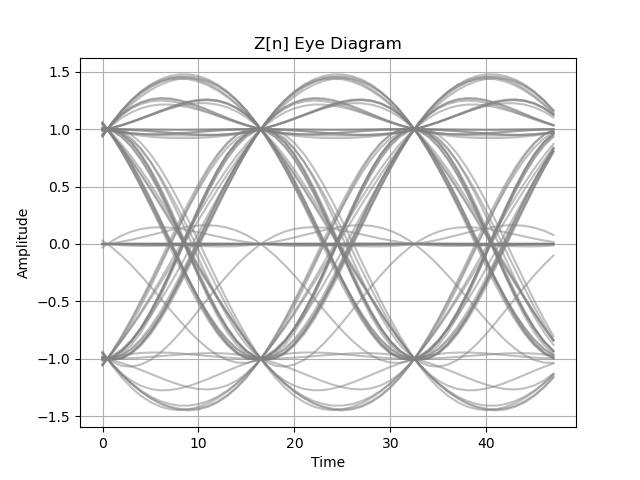
\includegraphics[width=1.2\textwidth]{assignment1a.png} % Include the figure
	\caption{Z-EyeDiagram}
	\label{fig:block}
\end{figure}

\begin{figure}[H] % [H] forces the figure to be placed exactly where it appears in the text
	\centering % Horizontally center the figure
	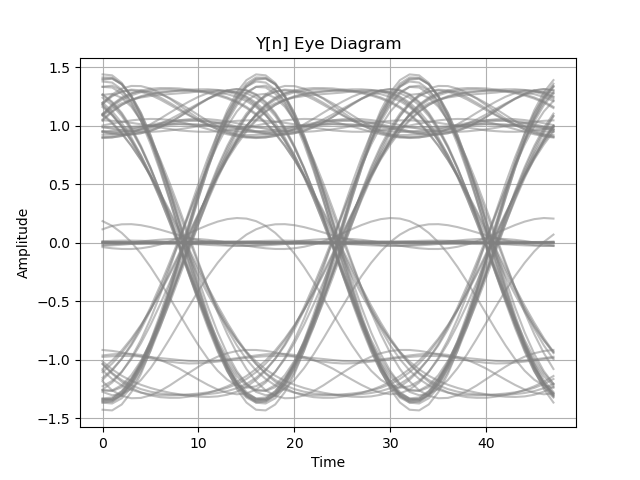
\includegraphics[width=1.2\textwidth]{assignment1b.png} % Include the figure
	\caption{Y-EyeDiagram}
	\label{fig:block}
\end{figure}

\begin{figure}[H] % [H] forces the figure to be placed exactly where it appears in the text
	\centering % Horizontally center the figure
	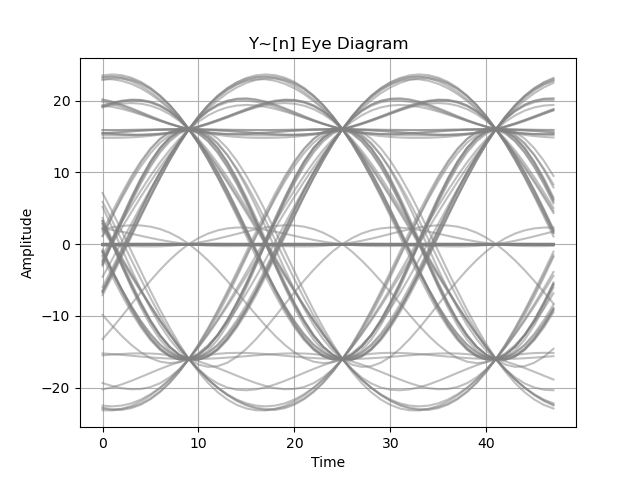
\includegraphics[width=1.2\textwidth]{assignment1c.png} % Include the figure
	\caption{YTilde-EyeDiagram}
	\label{fig:block}
\end{figure}

We see that Z[n] and Y~[n] Eye Diagrams are identical --disregarding timing offset. These signals are identical because Y~[n] is the product of (Y[n] or Root Raised Cosine Squared), which is equivalent to Raised Cosine or Z[n].


Root Raised Cosine or Y[n] suffers the most from ISI as compared to Raised Cosine or (Root Raised Cosine Squared). This is because Root Raised Cosine has the minimum distance between the '+1' Amplitude and '-1' Amplitude at the symbol decision point as compared to the other eye diagrams in Assignment 1.

\section{Assignment 2}

\begin{lstlisting}[language=Python]
	#################### PART TWO #######################
	def add_awgn(signal):
	"""Add Additive White Gaussian Noise (AWGN) to a signal."""
	noise_amplitude = 0.1
	noise = noise_amplitude * np.random.randn(len(signal))
	signal_noisy = signal + noise
	
	return signal_noisy
	
	# Add AWGN and create new eye diagrams
	z_n_noisy = add_awgn(z_n)
	y_n_noisy = add_awgn(y_n)
	y_tilde_n_noisy = add_awgn(y_tilde_n)
	
	plot_eye_diagram(z_n_noisy, sps, 'Z[n] + Noise Eye Diagram')
	plot_eye_diagram(y_n_noisy, sps, 'Y[n] + Noise Eye Diagram')
	plot_eye_diagram(y_tilde_n_noisy, sps, 'Y~[n] + Noise Eye Diagram')
	
\end{lstlisting}

\begin{figure}[H] % [H] forces the figure to be placed exactly where it appears in the text
	\centering % Horizontally center the figure
	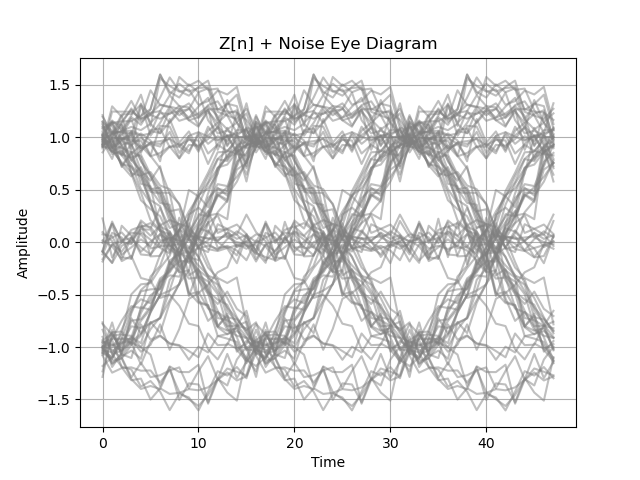
\includegraphics[width=1.2\textwidth]{assignment2a.png} % Include the figure
	\caption{Z+Noise - EyeDiagram}
	\label{fig:block}
\end{figure}

\begin{figure}[H] % [H] forces the figure to be placed exactly where it appears in the text
	\centering % Horizontally center the figure
	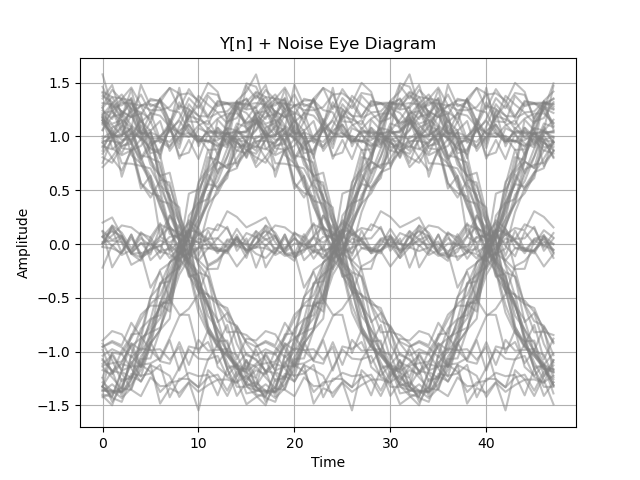
\includegraphics[width=1.2\textwidth]{assignment2b.png} % Include the figure
	\caption{Y+Noise - EyeDiagram}
	\label{fig:block}
\end{figure}

\begin{figure}[H] % [H] forces the figure to be placed exactly where it appears in the text
	\centering % Horizontally center the figure
	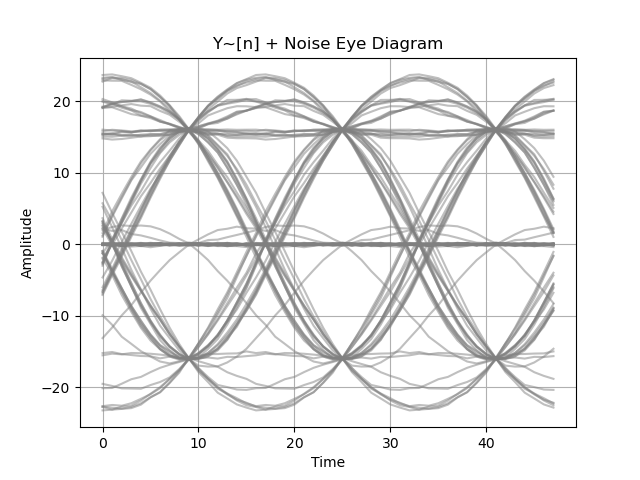
\includegraphics[width=1.2\textwidth]{assignment2c.png} % Include the figure
	\caption{YTilde+Noise - EyeDiagram}
	\label{fig:block}
\end{figure}

Clearly Y~[n] or (Root Raised Cosine Squared) has the highest SNR as compared to the other Eye diagrams in Assignment 2. This is because visually it is the least affected by noise.

\section{Assignment 3}

\begin{lstlisting}[language=Python]
	# Parameters
	sps = 16  # Samples per symbol (same as previous code)
	rx_matched = y_tilde_n  # Matched filter output from previous code
	
	# Simulate random timing offset
	h = np.zeros(sps)
	h[0] = 1
	h = np.roll(h, np.random.randint(sps))  # Apply random timing shift
	
	# Apply channel timing shift to the matched filter output
	rx_matched_shifted = np.convolve(rx_matched, h, mode='full')
	
	# Compute energy for each alignment offset
	energy = np.zeros(sps)
	for k in range(sps):
	# Compute energy for each offset by summing squared values of sampled segments
	energy[k] = np.sum(rx_matched_shifted[k::sps]**2)
	
	# Find the best offset
	max_ind = np.argmax(energy)
	
	# Align samples using max_ind
	rx_aligned = rx_matched_shifted[max_ind:]
	
	# Print results for verification
	print("Detected timing offset (max_ind):", max_ind)
	print("Energy values for each offset:", energy)
	
	# Verify if detected offset is within 2 samples of actual offset
	actual_offset = int(h.argmax())
	print("Actual timing offset:", actual_offset)
	print("Offset difference:", abs(max_ind - actual_offset))
	
	# Plot unaligned eye diagram (rx_matched_shifted)
	plot_eye_diagram(rx_matched_shifted, sps, 'Rx Matched Filter Before Offset')
	
	# Plot aligned eye diagram (rx_aligned)
	plot_eye_diagram(rx_aligned, sps, 'Rx Matched Filter After Offset')
\end{lstlisting}

\begin{lstlisting}[language=Python]
	Code Output:
	
	Detected timing offset (max ind): 7
	Energy values for each offset: [11786.44445008 12305.41667484 13082.15279012 13998.40271725
	14914.67659743 15691.48061124 16210.55427313 16392.85923999
	16210.65341876 15691.67562815 14914.93593006 13998.68583062
	13082.4156177  12305.61840032 11786.55378613 11604.24416745]
	Actual timing offset: 6
	Offset difference: 1
\end{lstlisting}

\begin{figure}[H] % [H] forces the figure to be placed exactly where it appears in the text
	\centering % Horizontally center the figure
	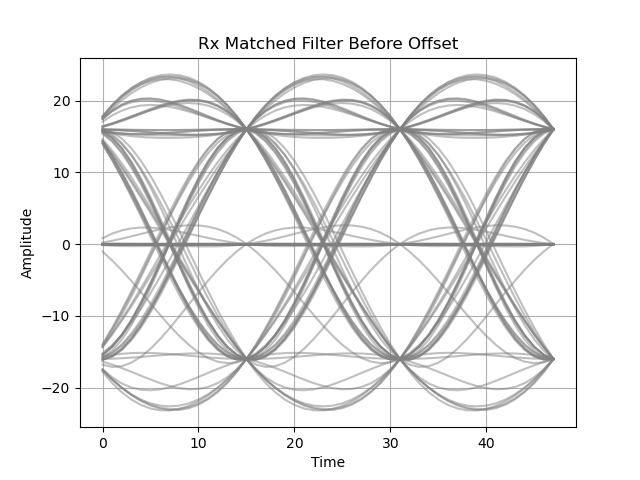
\includegraphics[width=1.2\textwidth]{assignment3a.png} % Include the figure
	\caption{RxMatchedFilterBeforeOffset}
	\label{fig:block}
\end{figure}

\begin{figure}[H] % [H] forces the figure to be placed exactly where it appears in the text
	\centering % Horizontally center the figure
	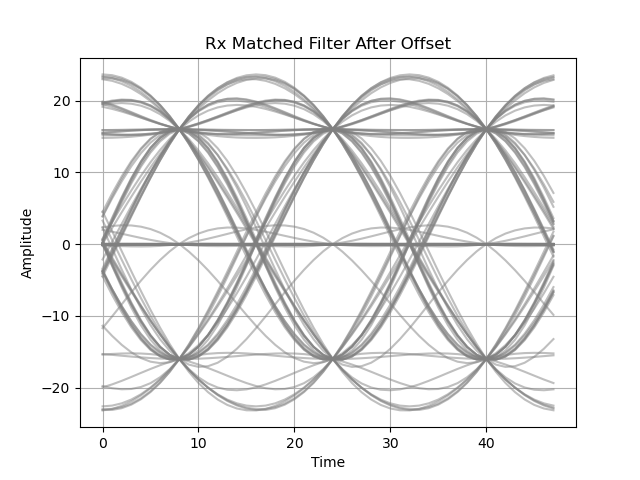
\includegraphics[width=1.2\textwidth]{assignment3b.png} % Include the figure
	\caption{RxMatchedFilterAfterOffset}
	\label{fig:block}
\end{figure}


\end{document}